%----------------------------------------------------------------------------------------
%	SLIDE 4.
%----------------------------------------------------------------------------------------
\begin{frame}
\frametitle{A big data számszerűen}

\begin{columns}
\begin{column}{0.45\textwidth}
	\begin{block}{\q{Small data}}
		\begin{itemize}
			\item \textit{Tabulae Rudolphinae} (1627): $1\,400$+ csillag pozíciójának adatai
			\item \textit{Histoire céleste française} (1801): $47\,390$ csillag pozíciója és magnitúdója
			\vspace{1.27em}
		\end{itemize}
	\end{block}
\end{column}
\begin{column}{0.45\textwidth}
    \begin{alertblock}{\q{Big data}}
		\begin{itemize}
			\item SDSS (2000--): $390\,292\,054$ fájl, $652$ TB adat
			\item EHT (2019): Az első \q{fotó} egy fekete lyukról, $5$ PB adat
			\item CERN: 500 exabyte (EB = $10^{3}$ PB) naponta (teljes mért adatmennyiség)
		\end{itemize}
	\end{alertblock}
\end{column}
\end{columns}

\begin{figure}
	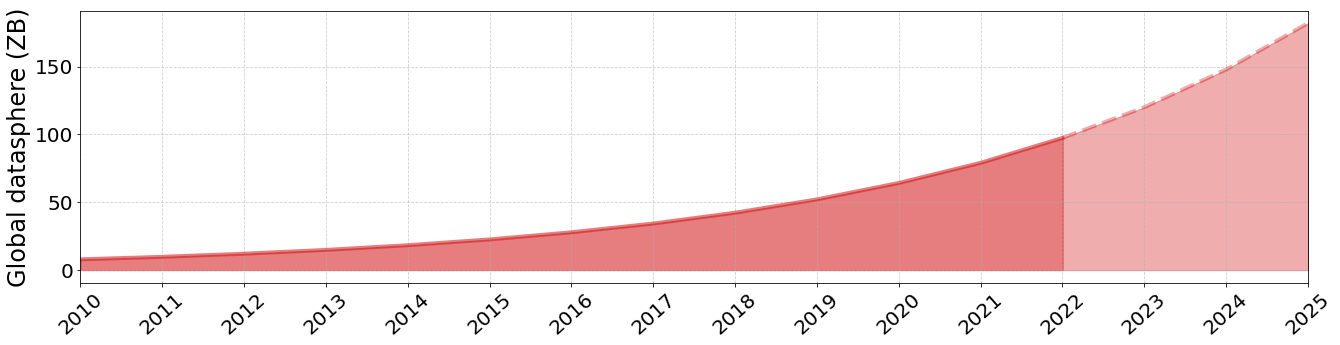
\includegraphics[width=1.0\textwidth]{img/data-boom.png}
\end{figure}

\end{frame}